\documentclass[sigconf]{acmart}
\settopmatter{printacmref=false}
\renewcommand\footnotetextcopyrightpermission[1]{}

\usepackage{graphicx}
\graphicspath{ {./Experiment Results/} }

\usepackage[backend=bibtex]{biblatex}
\addbibresource{References.bib}

\begin{document}
    \title{Ant Colony Optimisation for the Bin Packing Problem}
    \author{710018541}
    \maketitle
    
    \section{Literature Review}
        In the early 1990s, the development of metaheuristic approaches provided new ways to tackle complex optimisation problems that were previously difficult to solve. One of the most innovative techniques to emerge was Ant Colony Optimization (ACO), inspired by the behaviour of ant colonies, which efficiently find optimal solutions to complex problems through simple, decentralised processes. ACO has since been successfully applied to various challenges, including improving the efficiency of RFID antennas\cite{4426906}, optimising vehicle routing problems\cite{Emilio2004AntCO}, and as we will see here to the Bin Packing Problem.\newline
        
        Focusing on ant colony optimisation it is important to have a clear understanding of the basic approach we will be taking, which will be similar to that outlined in Marco Dorigo's paper on Ant Algorithms for Discrete Optimization\cite{10.1162/106454699568728}. This approach breaks problems down into three key steps which are repeated until some termination criteria is fulfilled; traversing the graph, evaporating pheromone, and setting pheromone\newline

        EXAMPLES OF ACO APPROACHES\newline

        The Bin Packing Problem, which we will be solving using our implementation of ACO, is a general problem-solving challenge that takes multiple different forms with the same underlying principle. Some focus on minimising the number of bins used to store the items such as that outlined in Towards Bin Packing (preliminary problem survey, models with multiset estimates)\cite{Levin2016TowardsBP}. Others like ours focus on some idea distribution of items (in our case the goal distribution will be that which minimises the difference in weights between the heaviest and lightest bins).\newline

        EXAMPLES OF BPP APPROACHES

    \section{Description of Results}
        \subsection{Experimental Setup}
            As part of any experiment it essential to have a clear idea of what the we are measuring and comparing, and how the experimental setup will affect these results. To this end, we have outlined our approach below along with reasoning for many of the decisions taken. We will commence by outlining our experiment's measurements, experimental variables, and control variables.\newline

            To assess the performance of each experimental run, we will measure:
            \begin{itemize}
                \item \textbf{Best solution fitness over time} - observes the algorithm’s peak performance in each iteration.
                \item \textbf{Average solution fitness over time} - indicates overall population performance and algorithm stability.
                \item \textbf{Standard deviation of fitness over time} - provides insight into population diversity, showing how converged or exploratory the population is over time.
            \end{itemize}
            
            Each of these metrics will be averaged across multiple trials for statistical robustness.\newline
            
            Our experimental variables which we will alter throughout:
            \begin{itemize}
                \item Ant population
                \item Evaporation rate\newline
            \end{itemize}

            And lastly our control variables which we wish to keep consistent throughout:
            \begin{itemize}
                \item Initial pheromone matrix
                \item Item choice given the same probabilities in time\newline
            \end{itemize}

            To ensure consistency, we will seed random functions (random and numpy.random) so that comparable trials yield consistent initial conditions. This seeding approach ensures that:
            \begin{itemize}
                \item The initial pheromone matrix (generated using random.uniform) is identical across comparable trials, enabling fair comparison.
                \item Two ants arriving at the same decision point (i.e. choosing which bin to assign to a given item) under identical conditions will make the same choice, enhancing the experiment’s repeatability and consistency.\newline
            \end{itemize}

            In cases where an optimal solution is achieved (i.e. the weight difference between the heaviest and lightest bins is zero), we handle this edge case by setting all other paths' pheromone values to zero while setting the selected optimal path’s pheromone value to one. This adjustment allows the experiment to proceed, with ants exclusively choosing the optimal path for the remainder of the run.\newline

        \subsection{Experimental Setup}
            Please see attached copy of implementation code.
            
        \subsection{Experimental Results}
            From the results generated in the experiment described above we were able to plot the following charts, enabling us to compare the performance of our implementation of ACO for the BPP with various different experimental variable configurations. This was done for both experimental setups described in the project specification.\newpage

            \subsubsection{BPP1 Experiment Results}:\newline
                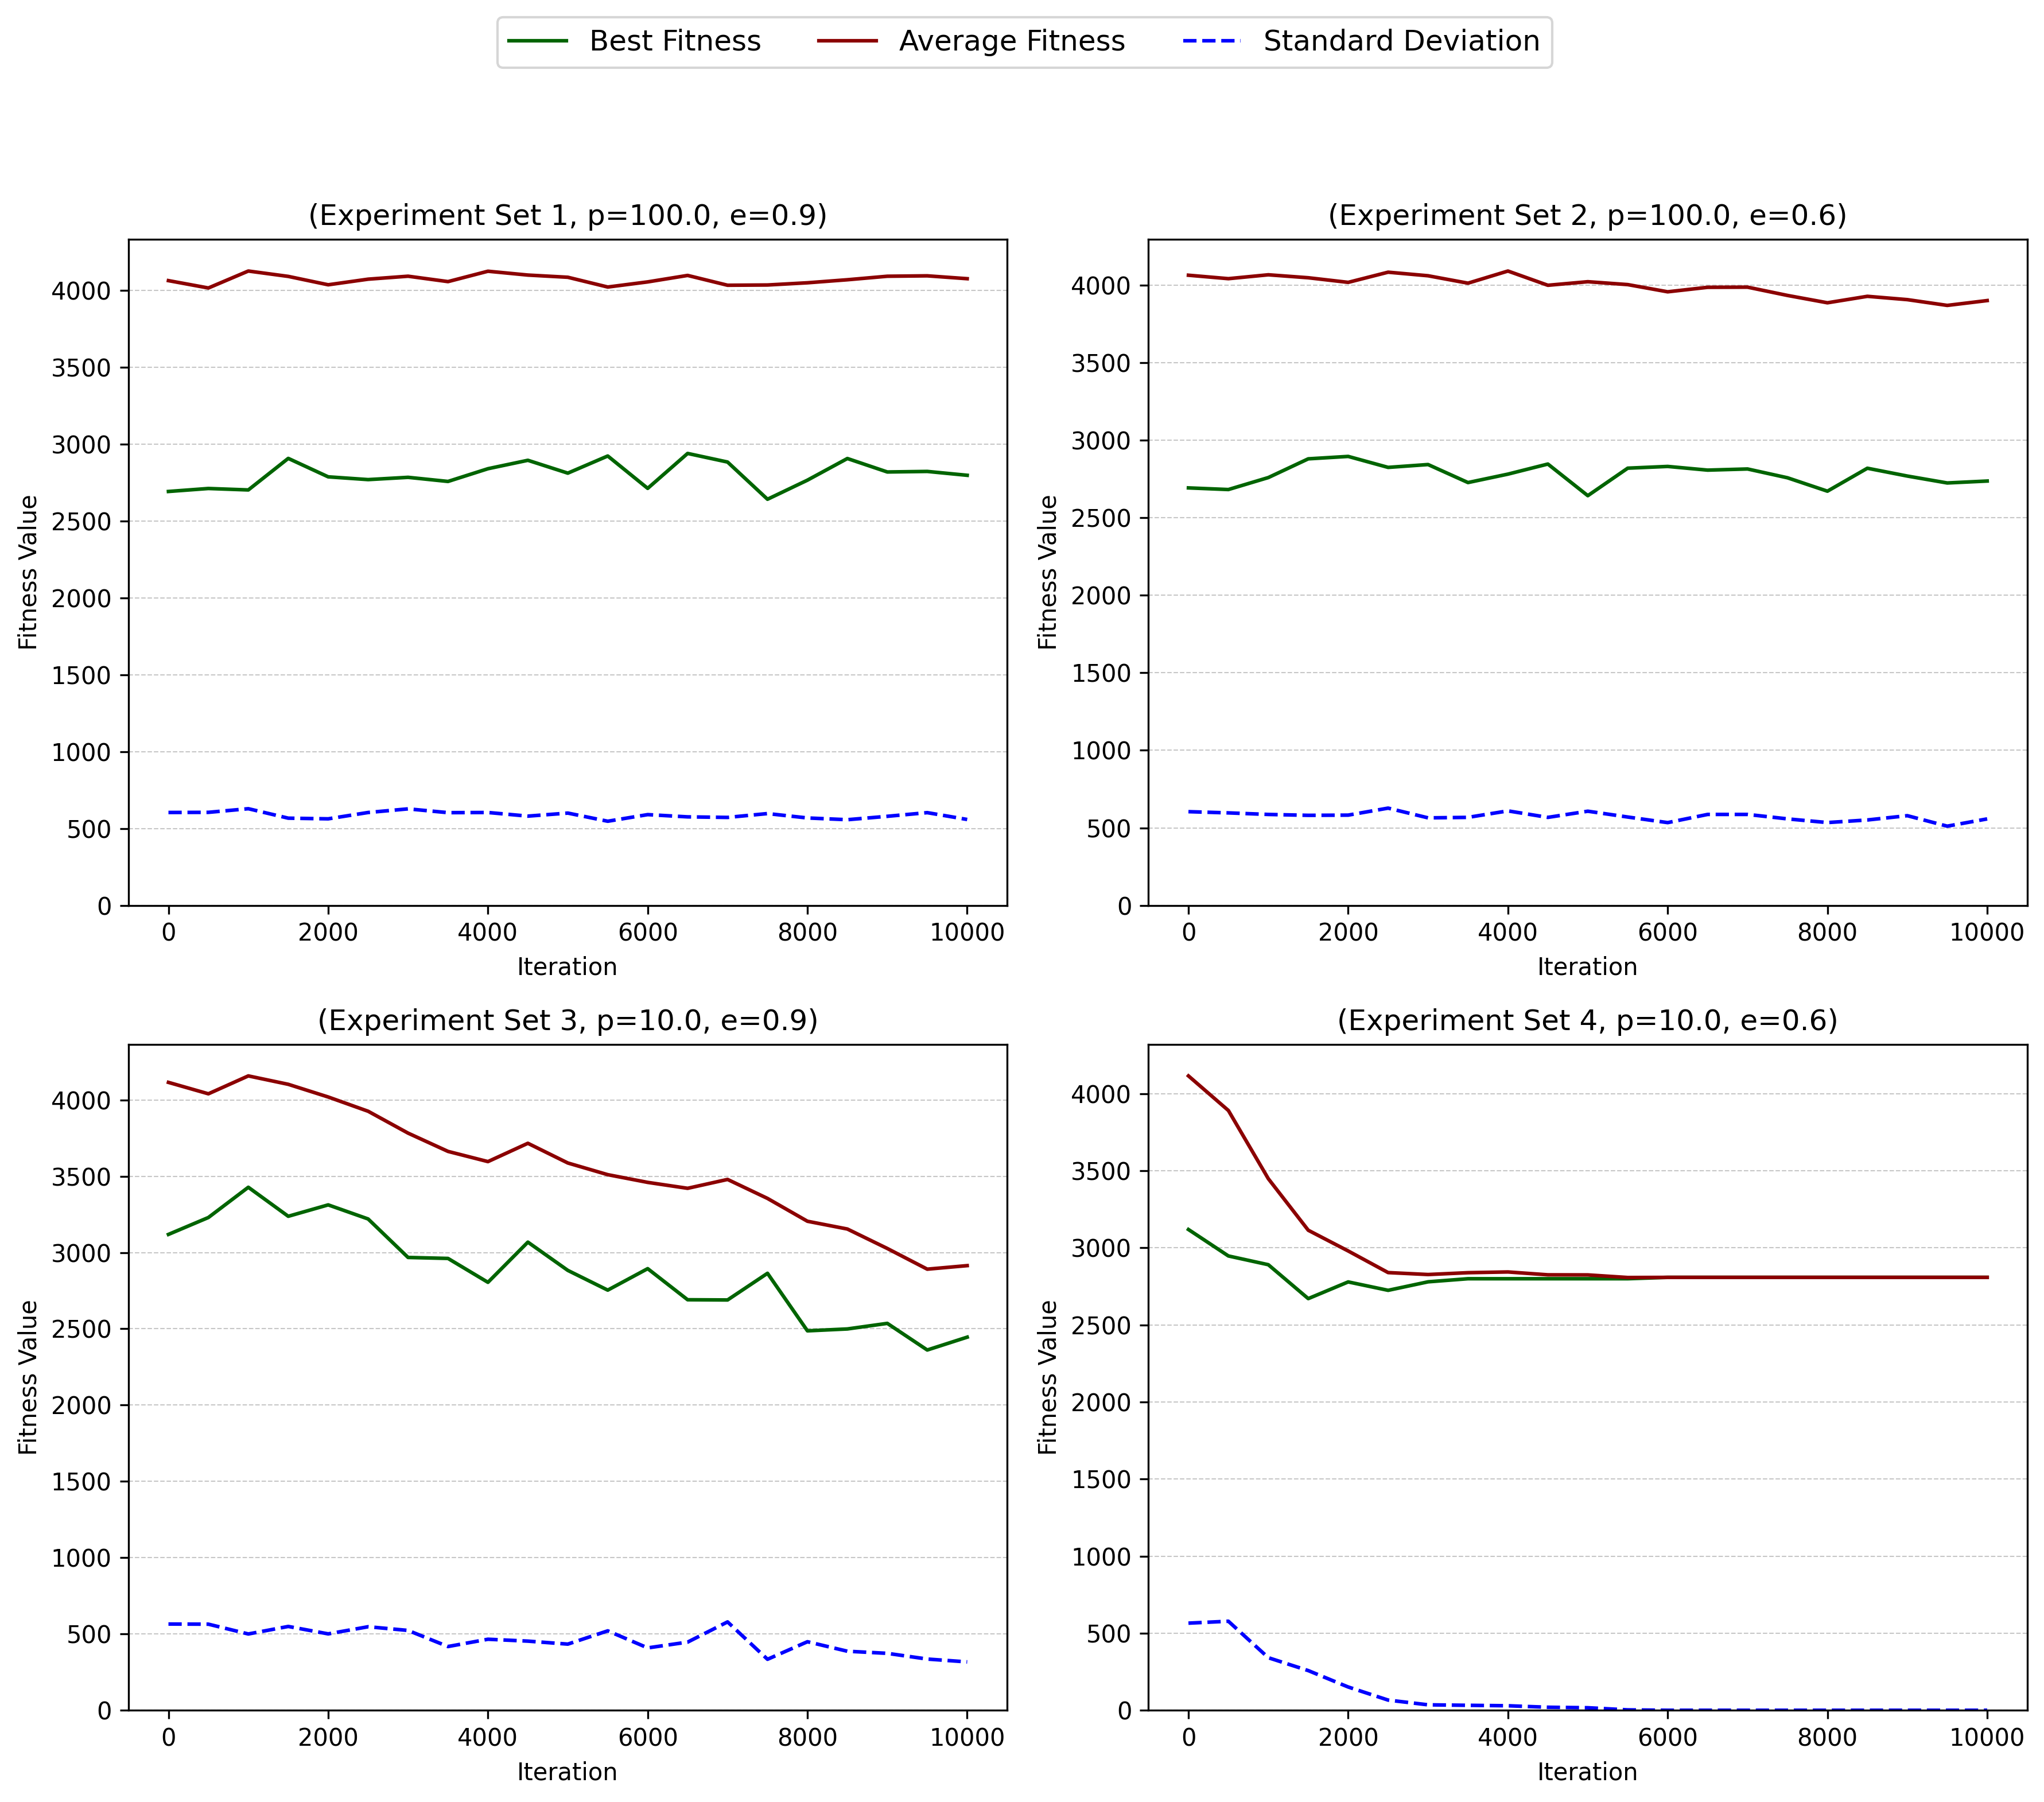
\includegraphics[scale=0.25]{Association for Computing Machinery (ACM) - SIG Proceedings Template/Experiment_Results/Experiment_BBP1_Metrics.png}\newline

            \subsubsection{BPP2 Experiment Results}:\newline
                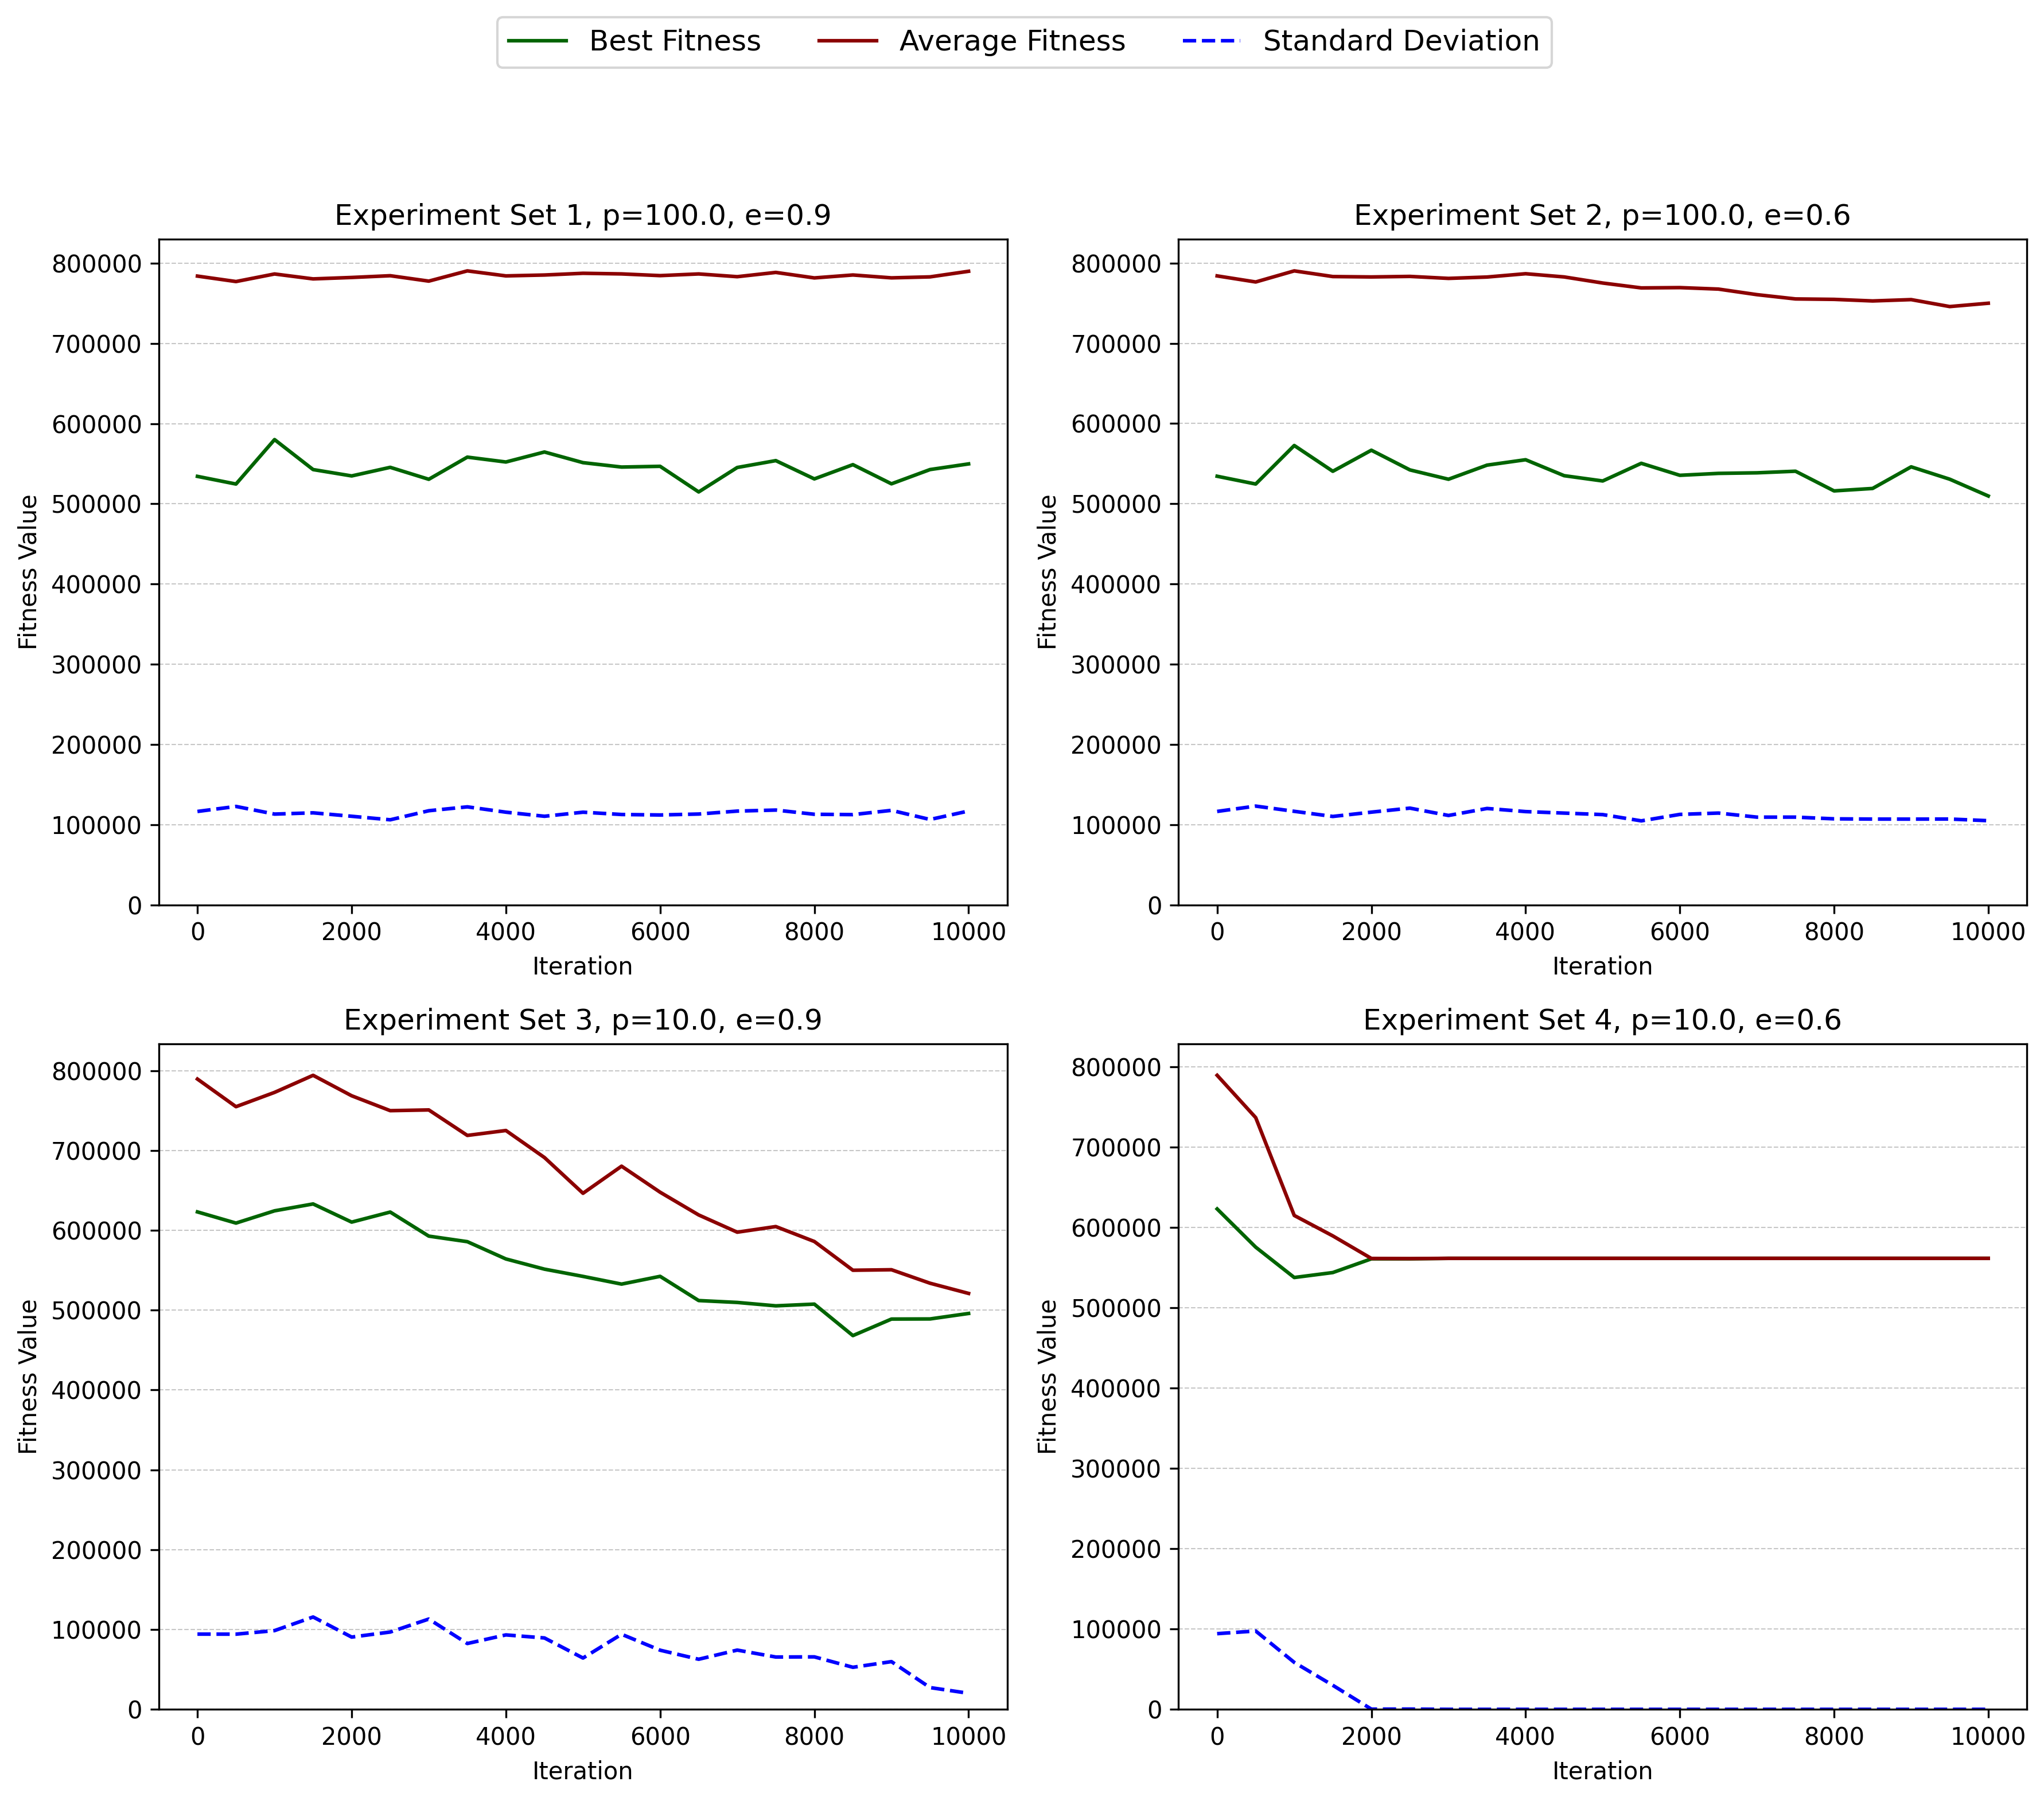
\includegraphics[scale=0.25]{Association for Computing Machinery (ACM) - SIG Proceedings Template/Experiment_Results/Experiment_BBP2_Metrics.png}\newline
            
            \textit{Description of the results of your experiments where tables and graphs of results should take up no more than 2 pages}

    \section{Discussion and Further Work}
        \textbf{DISCUSSION AND FURTHER WORK TO GO HERE}\newline
        Section including your answers to the following questions.
        \begin{itemize}
            \item \textbf{Question 1:} Which combination of parameters produces the best results?
            \item \textbf{Question 2:} What do you think is the reason for your findings in Question 1?
            \item \textbf{Question 3:} How do each of the parameter settings influence the performance of the algorithm?
            \item \textbf{Question 4:} Do you think that one of the algorithms in your literature review might have provided better results? Explain your answer.\newline
        \end{itemize}
        
        
        In your answers, describe your observations of the results, and describe any tentative explanations or conclusions you feel like making, and describe any further experiments you felt it interesting or useful to do.

    \printbibliography

\end{document}